\documentclass[11pt,a4paper]{article}
\usepackage{amsmath}\usepackage{amssymb}\usepackage[table]{xcolor}
\usepackage{tabularx}\usepackage{multirow}\usepackage{geometry}
\usepackage{enumitem}\usepackage{parskip}\usepackage{titlesec}
\usepackage{tocloft}\usepackage[most]{tcolorbox}
\usepackage{tikz}\usepackage{pgfplots}\pgfplotsset{compat=1.18}\usetikzlibrary{arrows.meta,calc,positioning,shapes.geometric,patterns}
\geometry{margin=2.5cm}
\titleformat{\section}{\large\bfseries}{}{0em}{}
\setlength{\cftbeforesecskip}{6pt}
\definecolor{q1color}{HTML}{D6EAF8}\definecolor{q2color}{HTML}{D5F5E3}
\definecolor{q3color}{HTML}{FDEBD0}\definecolor{q4color}{HTML}{F9E79F}
\definecolor{q5color}{HTML}{E8DAEF}\definecolor{q6color}{HTML}{FADBD8}
\definecolor{q7color}{HTML}{D1F2EB}\definecolor{q8color}{HTML}{FCF3CF}
\definecolor{q9color}{HTML}{EBDEF0}\definecolor{q10color}{HTML}{F5EEF8}
\newenvironment{mstab}[1]{%
  {\color{#1!75!black}\nobreak Mark Scheme}\par\nopagebreak\smallskip
  \arrayrulecolor{#1!70!black}\renewcommand{\arraystretch}{1.3}%
  \tabularx{\textwidth}{|>{\columncolor{#1!12}\raggedright\arraybackslash}p{1.9cm}|>{\columncolor{#1!12}}X|>{\columncolor{#1!12}\centering\arraybackslash}p{1.1cm}|}%
  \hline\rowcolor{#1!45} Question & Answer & Marks \\ \hline}{%
  \endtabularx\arrayrulecolor{black}\par\medskip}
\newtcolorbox{ansbox}[1]{colback=#1!8,colbacktitle=#1!30,colframe=#1!70!black,coltitle=black,fonttitle=\normalfont,title=Worked Solution,boxrule=0.6pt,arc=2mm,left=4pt,right=4pt,top=4pt,bottom=4pt,breakable}
\newcommand{\topiclabel}[1]{\hfill\normalfont\small\itshape\textcolor{black!55}{#1}}
\newcommand{\examq}[4]{\section[#1 - Q#2]{#1 - Q#2 - #3 - #4}}
\begin{document}
\begin{center}
  {\LARGE \textbf{Cambridge O Level Mathematics (Syllabus D) 4024/21/O/N/24}}\\[6pt]
  {\large October/November 2024 -- Mark Scheme \& Worked Solutions}
\end{center}
\bigskip

%========================= Q1 =========================
\examq{4024/21/O/N/24}{1}{Percentages Fundamentals \textperiodcentered\ Simple \& Compound Interest, Growth \& Decay \textperiodcentered\ Time, Currency \& Conversions}{11}

\begin{mstab}{q1color}
1(a) & 56.5 oe & 1 \\ \hline
1(b) & 17.2[0] cao \newline M1 for $5 \times 30 \times 13.45$ \newline M1 for $\dfrac{3324.70 - \text{their } 2017.50}{2 \times 38}$ & 3 \\ \hline
1(c) & 8.85 final answer \newline M3 for $\dfrac{245 \times 1.39}{50 \times 0.77}$ oe \newline OR M2 for $\dfrac{245 \times 1.39}{50}$ or $\dfrac{245}{50 \times 0.77}$ or $\dfrac{245 \times 1.39}{0.77}$ \newline OR M1 for $\dfrac{245}{0.77}$ or $\dfrac{\text{their amount in £}}{0.77}$ seen \newline and M1 for their $6.36 + \dfrac{39}{100} \times$ their $6.36$ seen & 4 \\ \hline
1(d) & 5284.50 \newline M2 for $12000\left(1 + \dfrac{1.5}{100}\right)^{4} + 12000\left(1 + \dfrac{1.5}{100}\right)^{3}$ \newline or for $24180 \times \left(1 + \dfrac{1.5}{100}\right)^{3}$ oe \newline or M1 for $12000\left(1 + \dfrac{1.5}{100}\right)^{k}$ oe, $k = 3$ or 4 ISW \newline After 0 scored, SC1 for $24180\left(1 + \dfrac{1.5}{100}\right)^{4}$ & 3 \\ \hline
\end{mstab}

\begin{ansbox}{q1color}
\textbf{(a)} Work out each type of day separately.
\[ 1030 \to 1800 = 7\tfrac{1}{2} \text{ hours, on 5 days: } 5 \times 7.5 = 37.5 \]
\[ 1000 \to 1930 = 9\tfrac{1}{2} \text{ hours, on 2 days: } 2 \times 9.5 = 19 \]
\[ 37.5 + 19 = 56.5 \text{ hours} \]

\textbf{(b)} First find what the sales assistants are paid in total.
\[ 5 \times 30 \times 13.45 = 150 \times 13.45 = 2017.50 \]
The rest of the wage bill goes to the two supervisors.
\[ 3324.70 - 2017.50 = 1307.20 \]
Between them the supervisors work $2 \times 38 = 76$ hours.
\[ \frac{1307.20}{76} = 17.20 \]
Each supervisor is paid $\$17.20$ per hour.

\textbf{(c)} Convert the total cost into dollars first. Since $\$1 = \pounds 0.77$, divide by $0.77$.
\[ \frac{245}{0.77} = 318.1818\ldots \text{ dollars for 50 games} \]
\[ \text{cost of one game} = \frac{318.1818\ldots}{50} = 6.3636\ldots \]
A profit of $39\%$ means the selling price is $139\%$ of the cost.
\[ 6.3636\ldots \times 1.39 = 8.8454\ldots \]
To the nearest cent the selling price is $\$8.85$.

\textbf{(d)} Each amount grows by a factor of $1.015$ for every complete year it is in the account.

The first $\$12\,000$ is in for all $4$ years:
\[ 12000 \times (1.015)^{4} = 12000 \times 1.0613635\ldots = 12\,736.36\ldots \]
The second $\$12\,000$ goes in at the end of year 1, so it earns interest for $3$ years:
\[ 12000 \times (1.015)^{3} = 12000 \times 1.0456783\ldots = 12\,548.14\ldots \]
Add these, then take out the $\$20\,000$.
\[ 12736.36\ldots + 12548.14\ldots = 25\,284.50\ldots \]
\[ 25284.50\ldots - 20000 = 5284.50 \]
The amount remaining is $\$5284.50$.
\end{ansbox}

%========================= Q2 =========================
\examq{4024/21/O/N/24}{2}{Statistical Diagrams \textperiodcentered\ Histograms}{7}

\begin{mstab}{q2color}
2(a)(i) & 162 \newline 108 \newline B1 for one correct \newline or M1 for $360 - 90 - $ their first angle \newline or M1 for $\dfrac{k \times 360}{160}$ oe or $\dfrac{360}{160} \times k$ where $k = 72$ or 48 \newline or M1 for $\dfrac{48}{40} \times 90$ oe or $\dfrac{72}{40} \times 90$ oe & 2 \\ \hline
2(a)(ii) & Correct pie chart \newline FT their angles adding to $270^{\circ}$ & 1 \\ \hline
2(b)(i) & Data grouped so individual speeds not known oe & 1 \\ \hline
2(b)(ii) & 46\quad 44\quad 38\quad 28 \newline B2 for 3 correct \newline or B1 for 2 correct & 3 \\ \hline
\end{mstab}

\begin{ansbox}{q2color}
\textbf{(a)(i)} The bottom row gives the scale: $40$ vehicles are shown by $90^{\circ}$.
\[ 1 \text{ vehicle} = \frac{90}{40} = 2.25^{\circ} \]
Multiply each remaining frequency by $2.25$.
\[ 72 \times 2.25 = 162^{\circ} \qquad 48 \times 2.25 = 108^{\circ} \]
Check: $162 + 108 + 90 = 360$ \checkmark, and $72 + 48 + 40 = 160$ vehicles \checkmark

\textbf{(a)(ii)} Measure the two new angles from the edge of the sector already drawn.

\begin{center}
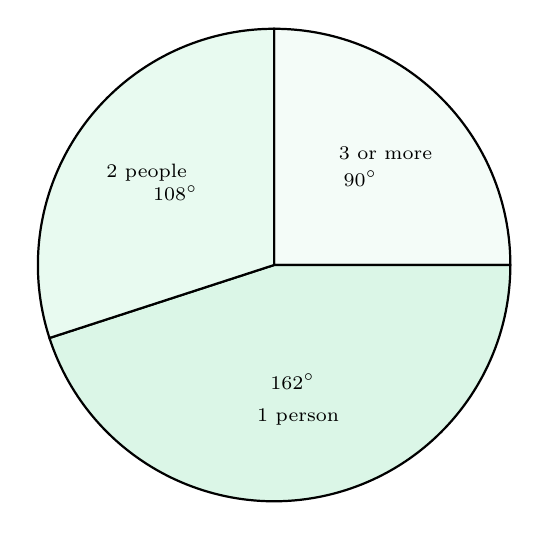
\begin{tikzpicture}[scale=1]
  \filldraw[fill=q2color!25, draw=black, thick] (0,0) -- (0:3) arc (0:90:3) -- cycle;
  \filldraw[fill=q2color!85, draw=black, thick] (0,0) -- (-162:3) arc (-162:0:3) -- cycle;
  \filldraw[fill=q2color!55, draw=black, thick] (0,0) -- (-270:3) arc (-270:-162:3) -- cycle;
  \node[font=\scriptsize] at (45:2.0) {3 or more};
  \node[font=\scriptsize] at (45:1.55) {$90^{\circ}$};
  \node[font=\scriptsize] at (-81:1.95) {1 person};
  \node[font=\scriptsize] at (-81:1.5) {$162^{\circ}$};
  \node[font=\scriptsize] at (144:2.0) {2 people};
  \node[font=\scriptsize] at (144:1.55) {$108^{\circ}$};
\end{tikzpicture}
\end{center}

\textbf{(b)(i)} A histogram shows only how many vehicles fall in each speed band, not the speed of any individual vehicle. The slowest vehicle could be anywhere in the lowest band and the fastest anywhere in the highest, so the range cannot be read off exactly. \textbf{The data is grouped, so the individual speeds are not known.}

\textbf{(b)(ii)} Each frequency is the area of its bar, so
\[ \text{frequency} = \text{frequency density} \times \text{class width} \]
Reading each bar height from the histogram and multiplying by its width gives
\begin{center}
\begin{tabular}{|c|c|c|c|}
\hline
Interval & Width & Frequency density & Frequency \\ \hline
$20 < s \leqslant 30$ & 10 & 2.4 & 24 \\ \hline
$30 < s \leqslant 40$ & 10 & 4.6 & 46 \\ \hline
$40 < s \leqslant 45$ & 5 & 8.8 & 44 \\ \hline
$45 < s \leqslant 50$ & 5 & 7.6 & 38 \\ \hline
$50 < s \leqslant 70$ & 20 & 1.4 & 28 \\ \hline
\end{tabular}
\end{center}
The first frequency, $24$, is already given, so the four to find are $46$, $44$, $38$ and $28$. Note that the two narrow bands in the middle are the tallest but not the fullest: the wide $50$ to $70$ band holds $28$ vehicles despite being the shortest bar.
\end{ansbox}

%========================= Q3 =========================
\examq{4024/21/O/N/24}{3}{Quadratic Graphs}{9}

\begin{mstab}{q3color}
3(a) & $-2$\quad $-2$ \newline B1 for each & 2 \\ \hline
3(b) & Correct smooth curve \newline B2FT for 8 or 9 points correctly plotted \newline or B1FT for 6 or 7 points correctly plotted & 3 \\ \hline
3(c) & $x = 2$ & 1 \\ \hline
3(d) & Correct ruled line \newline B1 for short or unruled line \newline or for two correct coordinates soi \newline or for line with positive gradient passing through $(0, 2)$ \newline or for line with gradient $\dfrac{1}{3}$ & 2 \\ \hline
3(e) & STRICT FT $x$-coordinates of intersection of their ruled line and their curve & 1 \\ \hline
\end{mstab}

\begin{ansbox}{q3color}
\textbf{(a)} Substitute the two missing values into $y = 4 + 2x - \dfrac{x^2}{2}$.
\[ x = -2: \quad y = 4 + 2(-2) - \frac{(-2)^2}{2} = 4 - 4 - 2 = -2 \]
\[ x = 6: \quad y = 4 + 2(6) - \frac{6^2}{2} = 4 + 12 - 18 = -2 \]
The completed table is
\begin{center}
\begin{tabular}{|c|c|c|c|c|c|c|c|c|c|}
\hline
$x$ & $-2$ & $-1$ & 0 & 1 & 2 & 3 & 4 & 5 & 6 \\ \hline
$y$ & $-2$ & 1.5 & 4 & 5.5 & 6 & 5.5 & 4 & 1.5 & $-2$ \\ \hline
\end{tabular}
\end{center}

\textbf{(b)} Plot the nine points and join them with a single smooth curve. The $x^2$ term is negative, so the curve is a downward parabola with its highest point at $(2, 6)$.

\textbf{(c)} A parabola is symmetrical about the vertical line through its highest point. The table is symmetrical about $x = 2$ (the values either side pair up: $1.5$ with $1.5$, $4$ with $4$, $5.5$ with $5.5$).
\[ x = 2 \]

\textbf{(d)} Rearrange $3y = x + 6$ into the form $y = mx + c$.
\[ y = \frac{x}{3} + 2 \]
So the line has gradient $\tfrac{1}{3}$ and passes through $(0, 2)$. Two convenient points to plot are $(0, 2)$ and $(6, 4)$; rule the line between them and extend it across the whole grid.

\begin{center}
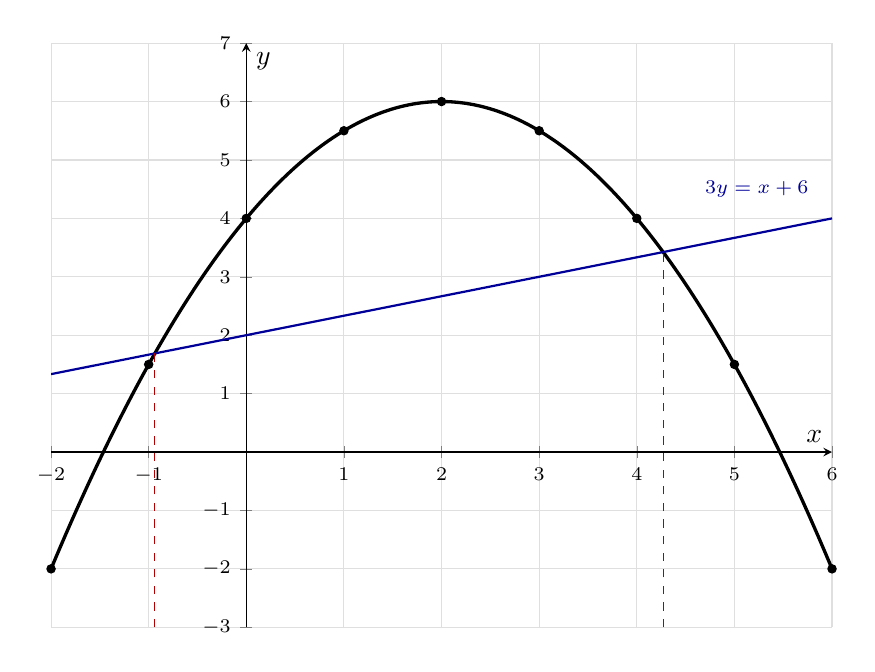
\begin{tikzpicture}
\begin{axis}[
  width=11.5cm, height=9cm,
  axis lines=middle,
  xmin=-2, xmax=6, ymin=-3, ymax=7,
  xtick={-2,-1,1,2,3,4,5,6}, ytick={-3,-2,-1,1,2,3,4,5,6,7},
  xlabel={$x$}, ylabel={$y$},
  grid=both, grid style={gray!25},
  tick label style={font=\scriptsize},
  clip=true]
  \addplot[very thick, smooth, domain=-2:6, samples=200]{4 + 2*x - x^2/2};
  \addplot[only marks, mark=*, mark size=1.5pt]
    coordinates {(-2,-2) (-1,1.5) (0,4) (1,5.5) (2,6) (3,5.5) (4,4) (5,1.5) (6,-2)};
  \addplot[thick, blue!60!black, domain=-2:6]{x/3 + 2};
  \draw[dashed, red!70!black] (axis cs:-0.937,-3) -- (axis cs:-0.937,1.688);
  \draw[dashed, red!70!black] (axis cs:4.271,-3) -- (axis cs:4.271,3.424);
  \node[anchor=west, font=\scriptsize, blue!60!black] at (axis cs:4.6,4.5) {$3y = x + 6$};
\end{axis}
\end{tikzpicture}
\end{center}

\textbf{(e)} Read off where the ruled line cuts the curve.
\[ x \approx -0.9 \qquad \text{and} \qquad x \approx 4.3 \]
(Algebraically these are the roots of $3x^2 - 10x - 12 = 0$, namely $-0.937\ldots$ and $4.271\ldots$, so any reading close to these from the candidate's own graph is accepted.)
\end{ansbox}

%========================= Q4 =========================
\examq{4024/21/O/N/24}{4}{Set Notation \& Venn Diagrams}{5}

\begin{mstab}{q4color}
4(a) & 3, 6, 9, 12, 15 & 1 \\ \hline
4(b) & $A$ only: 9, 12 \newline $A \cap B$: 3, 6, 15 \newline $B$ only: 1, 2, 5, 10 \newline Outside: 4, 7, 8, 11, 13, 14 \newline B1 for Venn diagram with 1 or 2 errors, omissions or repeats \newline or for correct Venn diagram with $(A \cup B)'$ blank & 2 \\ \hline
4(c) & 4 \newline FT their Venn diagram & 1 \\ \hline
4(d) & 2 \newline FT their Venn diagram & 1 \\ \hline
\end{mstab}

\begin{ansbox}{q4color}
The universal set is every integer from $1$ to $15$ inclusive.

\textbf{(a)} $A$ is the multiples of $3$ in that range.
\[ A = \{3,\ 6,\ 9,\ 12,\ 15\} \]

\textbf{(b)} $B$ is the factors of $30$ in that range. The factors of $30$ are $1, 2, 3, 5, 6, 10, 15, 30$, and $30$ is outside the range.
\[ B = \{1,\ 2,\ 3,\ 5,\ 6,\ 10,\ 15\} \]
Now sort the fifteen integers into the four regions.
\begin{itemize}[nosep,leftmargin=*]
  \item In both $A$ and $B$: $3$, $6$, $15$.
  \item In $A$ only: $9$, $12$.
  \item In $B$ only: $1$, $2$, $5$, $10$.
  \item In neither: $4$, $7$, $8$, $11$, $13$, $14$.
\end{itemize}
Every integer from $1$ to $15$ must appear exactly once, including those outside both circles.

\begin{center}
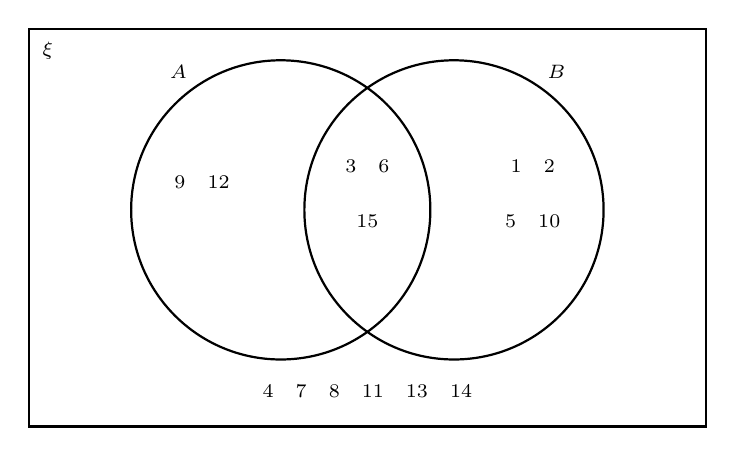
\begin{tikzpicture}[scale=1]
  \draw[thick] (-4.3,-2.75) rectangle (4.3,2.3);
  \node[anchor=north west, font=\scriptsize] at (-4.25,2.25) {$\xi$};
  \draw[thick] (-1.1,0) circle (1.9);
  \draw[thick] (1.1,0) circle (1.9);
  \node[anchor=south, font=\scriptsize] at (-2.4,1.55) {$A$};
  \node[anchor=south, font=\scriptsize] at (2.4,1.55) {$B$};
  \node[font=\scriptsize] at (-2.1,0.35) {9\quad 12};
  \node[font=\scriptsize] at (0,0.55) {3\quad 6};
  \node[font=\scriptsize] at (0,-0.15) {15};
  \node[font=\scriptsize] at (2.1,0.55) {1\quad 2};
  \node[font=\scriptsize] at (2.1,-0.15) {5\quad 10};
  \node[font=\scriptsize] at (0,-2.3) {4\quad 7\quad 8\quad 11\quad 13\quad 14};
\end{tikzpicture}
\end{center}

\textbf{(c)} $(A \cup B)'$ is everything outside both circles, that is $\{4, 7, 8, 11, 13, 14\}$. The smallest of these is
\[ x = 4 \]

\textbf{(d)} $A \cap B'$ means in $A$ but not in $B$, which is the ``$A$ only'' region $\{9, 12\}$.
\[ n(A \cap B') = 2 \]
\end{ansbox}

%========================= Q5 =========================
\examq{4024/21/O/N/24}{5}{Expanding \& Factorising Brackets \textperiodcentered\ Linear Equations \& Inequalities \textperiodcentered\ Rearranging Formulas \textperiodcentered\ Algebraic Fractions}{13}

\begin{mstab}{q5color}
5(a)(i) & 32 & 1 \\ \hline
5(a)(ii) & $-\dfrac{3}{2}$ oe final answer \newline M1 for $3 - 12 = 2x + 4x$ or better \newline or $-2x - 4x = 12 - 3$ or better & 2 \\ \hline
5(b)(i) & 41.8 oe \newline M1 for $5 \times 6.2 - 6 \times (-1.8)$ oe & 2 \\ \hline
5(b)(ii) & $\dfrac{w + 6y}{5}$ oe final answer \newline M1 for $w + 6y = 5x$ or $x = \dfrac{w}{5} - \dfrac{6y}{5}$ or $-5x = -6y - w$ & 2 \\ \hline
5(c) & $(5 - x)(3y + x)$ or $-(x - 5)(3y + x)$ final answer \newline B1 for one correct partial factorisation seen & 2 \\ \hline
5(d) & $\dfrac{x^2 - 2x + 9}{(x - 3)(x + 3)}$ final answer or $\dfrac{x^2 - 2x + 9}{x^2 - 9}$ final answer \newline B2 for $2x + 6 - 4x + 12 + x^2 + 3x - 3x - 9$ oe isw \newline or B1 for $2(x + 3) - 4(x - 3) + (x - 3)(x + 3)$ oe isw \newline B1 for denominator $(x - 3)(x + 3)$ oe isw \newline After 0 scored, SC1 for $\dfrac{2(x + 3) - 4(x - 3)}{(x + 3)(x - 3)}$ oe isw or $\dfrac{-x + 3 + 4}{x + 3}$ oe isw or $\dfrac{2x + 3 - 3}{x - 3}$ oe isw & 4 \\ \hline
\end{mstab}

\begin{ansbox}{q5color}
\textbf{(a)(i)} Multiply both sides by $4$.
\[ \frac{y}{4} = 8 \quad \Rightarrow \quad y = 32 \]

\textbf{(a)(ii)} Collect the $x$ terms on one side and the numbers on the other.
\[ 3 - 4x = 2x + 12 \]
\[ 3 - 12 = 2x + 4x \]
\[ -9 = 6x \]
\[ x = -\frac{9}{6} = -\frac{3}{2} \]

\textbf{(b)(i)} Substitute into $w = 5x - 6y$, taking care with the negative value of $y$.
\[ w = 5(6.2) - 6(-1.8) \]
\[ = 31 + 10.8 = 41.8 \]

\textbf{(b)(ii)} Make $x$ the subject of $w = 5x - 6y$.
\[ w + 6y = 5x \]
\[ x = \frac{w + 6y}{5} \]

\textbf{(c)} Factorise in pairs.
\[ 15y - 3xy - x^2 + 5x \]
Take $3y$ out of the first pair and $-x$ out of the second:
\[ = 3y(5 - x) - x(x - 5) \]
Note that $-x(x - 5) = x(5 - x)$, so both parts share the bracket $(5 - x)$.
\[ = 3y(5 - x) + x(5 - x) \]
\[ = (5 - x)(3y + x) \]

\textbf{(d)} The denominators are $x - 3$ and $x + 3$, so the common denominator is $(x - 3)(x + 3)$. The $+1$ must also be written over it.
\[ \frac{2}{x - 3} - \frac{4}{x + 3} + 1 = \frac{2(x + 3) - 4(x - 3) + (x - 3)(x + 3)}{(x - 3)(x + 3)} \]
Expand the numerator term by term.
\[ 2(x + 3) = 2x + 6 \]
\[ -4(x - 3) = -4x + 12 \]
\[ (x - 3)(x + 3) = x^2 - 9 \]
Add them and collect like terms.
\[ 2x + 6 - 4x + 12 + x^2 - 9 = x^2 - 2x + 9 \]
\[ = \frac{x^2 - 2x + 9}{(x - 3)(x + 3)} \]
The numerator does not factorise, so nothing cancels. The denominator may also be left expanded as $x^2 - 9$.
\end{ansbox}

%========================= Q6 =========================
\examq{4024/21/O/N/24}{6}{Volume \& Surface Area \textperiodcentered\ Congruence \& Similarity \textperiodcentered\ Pythagoras \& Trigonometry (Right-Angled)}{10}

\begin{mstab}{q6color}
6(a) & 180 or 179.5 to 179.6\ldots \newline M1 for (cube length)$^3 = 343$ oe \newline M1 for $\dfrac{4}{3}\pi\left(\text{their } 3.5\right)^{3}$ & 3 \\ \hline
6(b) & 20 \newline M1 for $\sqrt[3]{\dfrac{1280}{540}}$ oe or $\sqrt[3]{\dfrac{540}{1280}}$ oe or $\dfrac{15^3}{h^3} = \dfrac{540}{1280}$ oe & 2 \\ \hline
6(c) & 653 or 653.1 to 653.2\ldots \newline M1 for $\sqrt{8.7^2 - 6.3^2}$ \newline M1 for $\dfrac{3 \times \text{their } 6}{2}$ \newline M2 for $\pi \times 6.3 \times 8.7 + 2 \times \pi \times 6.3 \times \text{their } 9 + \pi \times 6.3^{2}$ \newline or M1 for $\pi \times 6.3 \times 8.7$ or $2\pi \times 6.3 \times \text{their } 9$ & 5 \\ \hline
\end{mstab}

\begin{ansbox}{q6color}
\textbf{(a)} The sphere touches all six faces, so its diameter equals the side of the cube.
\[ \text{(cube length)}^3 = 343 \quad \Rightarrow \quad \text{cube length} = \sqrt[3]{343} = 7\ \mathrm{cm} \]
\[ \text{radius of sphere} = \frac{7}{2} = 3.5\ \mathrm{cm} \]
\[ V = \frac{4}{3}\pi r^3 = \frac{4}{3}\pi (3.5)^3 = \frac{4}{3}\pi \times 42.875 \]
\[ = 179.59\ldots \]
The volume of the sphere is $180\ \mathrm{cm^3}$ (3 sf).

\textbf{(b)} For similar solids, volumes are in the ratio of the cube of the lengths.
\[ \frac{V_B}{V_A} = \frac{1280}{540} = \frac{64}{27} \]
\[ \frac{h_B}{15} = \sqrt[3]{\frac{64}{27}} = \frac{4}{3} \]
\[ h_B = \frac{4}{3} \times 15 = 20 \]
The height of solid $B$ is $20\ \mathrm{cm}$.

\textbf{(c)} The slant height, radius and vertical height of the cone form a right-angled triangle.
\[ \text{height of cone} = \sqrt{8.7^2 - 6.3^2} = \sqrt{75.69 - 39.69} = \sqrt{36} = 6\ \mathrm{cm} \]
The ratio of heights is $2 : 3$, so
\[ \text{height of cylinder} = \frac{3 \times 6}{2} = 9\ \mathrm{cm} \]
The surface of the solid is three parts: the curved cone, the curved cylinder, and the flat circular base. There is no circle where the cone meets the cylinder, because that join is inside the solid.
\[ \text{curved cone} = \pi r l = \pi \times 6.3 \times 8.7 = 172.18\ldots \]
\[ \text{curved cylinder} = 2\pi r h = 2 \times \pi \times 6.3 \times 9 = 356.24\ldots \]
\[ \text{base circle} = \pi r^2 = \pi \times 6.3^2 = 124.69\ldots \]
\[ \text{total} = 172.18\ldots + 356.24\ldots + 124.69\ldots = 653.11\ldots \]
The total surface area is $653\ \mathrm{cm^2}$ (3 sf).
\end{ansbox}

%========================= Q7 =========================
\examq{4024/21/O/N/24}{7}{Coordinate Geometry \textperiodcentered\ Linear Graphs \textperiodcentered\ Vectors}{10}

\begin{mstab}{q7color}
7(a) & $(-4, 1)$ & 1 \\ \hline
7(b) & 6.08 or 6.082 to 6.083 \newline M1 for $\sqrt{(-1)^2 + (-6)^2}$ oe & 2 \\ \hline
7(c) & $\begin{pmatrix} 4 \\ -8 \end{pmatrix}$ \newline B2 for one component correct \newline or B1 for [$C =$] $(1, -1)$ or $\begin{pmatrix} 5 \\ -2 \end{pmatrix}$ & 3 \\ \hline
7(d) & $y = \dfrac{5}{2}x + 11$ oe final answer \newline M1 for [gradient $AB =$] $\dfrac{5 - 7}{2 - -3}$ oe \newline M1 for [gradient $L =$] $\dfrac{-1}{\text{their gradient } AB}$ \newline M1 for their $(-4, 1)$ substituted into $y = \left(\text{their } \dfrac{5}{2}\right)x + c$ \newline or $y - 1 = \left(\text{their } \dfrac{5}{2}\right)(x - -4)$ & 4 \\ \hline
\end{mstab}

\begin{ansbox}{q7color}
\textbf{(a)} The vector $\overrightarrow{AD} = \begin{pmatrix} -1 \\ -6 \end{pmatrix}$ means $1$ left and $6$ down from $A(-3, 7)$.
\[ D = (-3 - 1,\ 7 - 6) = (-4,\ 1) \]

\textbf{(b)} The length of a vector comes from Pythagoras on its two components.
\[ AD = \sqrt{(-1)^2 + (-6)^2} = \sqrt{1 + 36} = \sqrt{37} \]
\[ = 6.082\ldots = 6.08 \]

\textbf{(c)} In the parallelogram $ABCD$ the sides $BC$ and $AD$ are equal and parallel, so $\overrightarrow{BC} = \overrightarrow{AD}$.
\[ \overrightarrow{AB} = \begin{pmatrix} 2 - (-3) \\ 5 - 7 \end{pmatrix} = \begin{pmatrix} 5 \\ -2 \end{pmatrix} \]
Going from $A$ to $B$ and then from $B$ to $C$:
\[ \overrightarrow{AC} = \overrightarrow{AB} + \overrightarrow{BC} = \begin{pmatrix} 5 \\ -2 \end{pmatrix} + \begin{pmatrix} -1 \\ -6 \end{pmatrix} = \begin{pmatrix} 4 \\ -8 \end{pmatrix} \]
(This puts $C$ at $(-3 + 4,\ 7 - 8) = (1, -1)$.)

\textbf{(d)} First the gradient of $AB$, from $A(-3, 7)$ to $B(2, 5)$.
\[ m_{AB} = \frac{5 - 7}{2 - (-3)} = \frac{-2}{5} \]
Perpendicular gradients multiply to $-1$.
\[ m_{L} = \frac{-1}{-\frac{2}{5}} = \frac{5}{2} \]
Line $L$ passes through $D(-4, 1)$, so substitute to find $c$.
\[ 1 = \frac{5}{2}(-4) + c \]
\[ 1 = -10 + c \quad \Rightarrow \quad c = 11 \]
\[ y = \frac{5}{2}x + 11 \]
\end{ansbox}

%========================= Q8 =========================
\examq{4024/21/O/N/24}{8}{Compound Measures \textperiodcentered\ Bearings, Constructions \& Scale Drawings \textperiodcentered\ Pythagoras \& Trigonometry (Right-Angled) \textperiodcentered\ Sine, Cosine Rule \& Area of Triangles}{8}

\begin{mstab}{q8color}
8(a) & 1.97[0\ldots] \newline M2 for $\dfrac{320 + 250}{\frac{320}{1.6} + \frac{250}{2.8}}$ \newline or M1 for $\dfrac{320}{1.6}$ or $\dfrac{250}{2.8}$ & 3 \\ \hline
8(b) & 195 or 194.79 to 194.81 \newline B4 for 48.19 to 48.3 \newline OR \newline M1 for $BD^2 = 132^2 + 250^2$ oe \newline M2 for $\cos B\hat{A}D = \dfrac{365^2 + 320^2 - \text{their } BD^2}{2 \times 365 \times 320}$ or better \newline or M1 for their $BD^2 = 365^2 + 320^2 - 2 \times 365 \times 320\cos B\hat{A}D$ \newline M1 for bearing $= 243 - $ their $B\hat{A}D$ & 5 \\ \hline
\end{mstab}

\begin{ansbox}{q8color}
\textbf{(a)} Average speed over the whole journey is total distance divided by total time, not the mean of the two speeds.
\[ \text{total distance} = 320 + 250 = 570\ \mathrm{m} \]
\[ \text{time } A \to B = \frac{320}{1.6} = 200\ \mathrm{s} \]
\[ \text{time } B \to C = \frac{250}{2.8} = 89.285\ldots\ \mathrm{s} \]
\[ \text{total time} = 200 + 89.285\ldots = 289.285\ldots\ \mathrm{s} \]
\[ \text{average speed} = \frac{570}{289.285\ldots} = 1.970\ldots \]
Ray's average speed is $1.97\ \mathrm{m/s}$ (3 sf).

\textbf{(b)} The bearing of $B$ from $A$ differs from the bearing of $D$ from $A$ by the angle $B\hat{A}D$, so that angle is what is needed.

Triangle $BCD$ is right-angled at $C$, so Pythagoras gives the diagonal $BD$.
\[ BD^2 = 250^2 + 132^2 = 62\,500 + 17\,424 = 79\,924 \]
\[ BD = 282.70\ldots\ \mathrm{m} \]
Now use the cosine rule in triangle $ABD$, where $AB = 320$ and $AD = 365$.
\[ \cos B\hat{A}D = \frac{365^2 + 320^2 - 79\,924}{2 \times 365 \times 320} \]
\[ = \frac{133\,225 + 102\,400 - 79\,924}{233\,600} = \frac{155\,701}{233\,600} = 0.66652\ldots \]
\[ B\hat{A}D = 48.21\ldots^{\circ} \]
$B$ lies anticlockwise of $D$ as seen from $A$, so subtract.
\[ \text{bearing of } B \text{ from } A = 243 - 48.21\ldots = 194.79\ldots \]
The bearing is $195^{\circ}$ (3 sf).
\end{ansbox}

%========================= Q9 =========================
\examq{4024/21/O/N/24}{9}{Angles in Polygons \& Parallel Lines \textperiodcentered\ Circle Theorems \textperiodcentered\ Pythagoras \& Trigonometry (Right-Angled) \textperiodcentered\ Sine, Cosine Rule \& Area of Triangles}{10}

\begin{mstab}{q9color}
 & $[x =]\ 98$ \newline B1 for $A\hat{B}E = 28$ or $A\hat{E}C = 126$ \newline or M1 for $180 - 54 - 28$ oe & B2 \\
\multirow{-2}{1.9cm}{9(a)} & $[y =]\ 72$ \newline B1 for $C\hat{E}D = 54$ or $E\hat{C}D = 54$ \newline or $C\hat{E}D = 180 - 28 - $ their $x$ oe & B2 \\ \hline
9(b) & 35.2 or 35.16 to 35.24 \newline B1 for $O\hat{R}Q = 90$ soi \newline B1 for $O\hat{Q}R = 20$ or $R\hat{O}Q = 70$ \newline M2 for [radius $=$] $12\tan$ their $20$ oe \newline or $PQ = \dfrac{12\sin\left(\text{their } P\hat{R}Q\right)}{\sin 35}$ oe \newline or $PR = \dfrac{12\sin\left(\text{their } 20\right)}{\sin 35}$ oe \newline or M1 for $\tan\left(\text{their } 20\right) = \dfrac{OR}{12}$ oe \newline M1 for $\dfrac{1}{2}\left(\text{their } OR\right)^2 \sin\left(180 - \text{their } 70\right) + \dfrac{1}{2}\left(\text{their } OR\right) \times 12$ \newline or $\dfrac{1}{2}\left(\text{their } OQ + \text{their } OP\right) \times 12 \times \sin\left(\text{their } 20\right)$ oe & 6 \\ \hline
\end{mstab}

\begin{ansbox}{q9color}
\textbf{(a)} The angle marked $x^{\circ}$ is the third angle of the triangle containing the $54^{\circ}$ and $28^{\circ}$ angles, and the angles of a triangle add to $180^{\circ}$.
\[ x = 180 - 54 - 28 = 98 \]

Because $AB$ is parallel to $EC$, the angle $A\hat{E}C$ comes out as $126^{\circ}$, and $A$, $E$, $D$ lie on a straight line, so
\[ C\hat{E}D = 180 - 126 = 54^{\circ} \]
(The same value follows from the triangle: $C\hat{E}D = 180 - 28 - x = 180 - 28 - 98 = 54$.)

Now use $CD = DE$. Triangle $CDE$ is isosceles with the two equal sides meeting at $D$, so the base angles at $C$ and at $E$ are equal.
\[ E\hat{C}D = C\hat{E}D = 54^{\circ} \]
\[ y = 180 - 54 - 54 = 72 \]

\textbf{(b)} $O$ lies on $PQ$, and $OP$ and $OR$ are both radii, so triangle $OPR$ is isosceles.
\[ O\hat{R}P = R\hat{P}O = 35^{\circ} \]
\[ P\hat{O}R = 180 - 35 - 35 = 110^{\circ} \]
$P$, $O$, $Q$ lie on a straight line, so
\[ R\hat{O}Q = 180 - 110 = 70^{\circ} \]
$QR$ is a tangent and $OR$ is a radius, so they meet at a right angle.
\[ O\hat{R}Q = 90^{\circ} \]
\[ O\hat{Q}R = 180 - 90 - 70 = 20^{\circ} \]
In right-angled triangle $ORQ$, with $QR = 12$,
\[ \tan 20^{\circ} = \frac{OR}{12} \quad \Rightarrow \quad OR = 12\tan 20^{\circ} = 4.3676\ldots\ \mathrm{cm} \]
This is the radius, so $OP = OR = 4.3676\ldots$ too.

Now split triangle $PQR$ into triangle $POR$ and triangle $ORQ$.
\[ \text{area } POR = \frac{1}{2}(OP)(OR)\sin 110^{\circ} = \frac{1}{2}(4.3676\ldots)^2 \sin 110^{\circ} = 8.961\ldots \]
\[ \text{area } ORQ = \frac{1}{2} \times OR \times QR = \frac{1}{2} \times 4.3676\ldots \times 12 = 26.205\ldots \]
\[ \text{total} = 8.961\ldots + 26.205\ldots = 35.16\ldots \]
The area of triangle $PQR$ is $35.2\ \mathrm{cm^2}$ (3 sf).
\end{ansbox}

%========================= Q10 =========================
\examq{4024/21/O/N/24}{10}{Quadratic Equations \textperiodcentered\ Forming \& Solving Equations \textperiodcentered\ Algebraic Fractions}{10}

\begin{mstab}{q10color}
 & $r + r + 6 = x$ oe & M1 \\
\multirow{-2}{1.9cm}{10(a)} & $r = \dfrac{x - 6}{2}$ leading to fraction red $= \dfrac{x - 6}{2x}$ \newline A0 if any errors or omissions & A1 \\ \hline
 & green in $A = \dfrac{x}{2} + 3$ oe \newline Allow green in $B = 4\left(\dfrac{x}{2} + 3\right)$ oe & M1 \\
\multirow{-2}{1.9cm}{10(b)} & Total in $B = x + 4\left(\dfrac{x}{2} + 3\right)$ oe leading to fraction red $= \dfrac{x}{3x + 12}$ & A1 \\ \hline
 & $(x - 6)(3x + 12) = 2x^2$ oe \newline Correct removal of fractions & M1 \\
 & $3x^2 - 18x + 12x - 72$ \newline Accept 3 out of 4 terms correct & M1 \\
\multirow{-3}{1.9cm}{10(c)} & Correct rearrangement to $x^2 - 6x - 72 = 0$ \newline A0 if any errors or omissions & A1 \\ \hline
 & $(x + 6)(x - 12) = 0$ & B1 \\
\multirow{-2}{1.9cm}{10(d)} & 12, $-6$ & B1 \\ \hline
10(e) & 9 \newline FT their positive solution $\div\ 2 + 3$ & 1 \\ \hline
\end{mstab}

\begin{ansbox}{q10color}
\textbf{(a)} Let the number of red balls in bag $A$ be $r$. The greens are $6$ more, so there are $r + 6$ of them, and the two together make up all $x$ balls.
\[ r + (r + 6) = x \]
\[ 2r = x - 6 \quad \Rightarrow \quad r = \frac{x - 6}{2} \]
The fraction that are red is the reds divided by the total.
\[ \frac{r}{x} = \frac{x - 6}{2} \div x = \frac{x - 6}{2x} \]

\textbf{(b)} The greens in bag $A$ number
\[ r + 6 = \frac{x - 6}{2} + 6 = \frac{x - 6 + 12}{2} = \frac{x + 6}{2} = \frac{x}{2} + 3 \]
Bag $B$ has $4$ times as many greens:
\[ \text{green in } B = 4\left(\frac{x}{2} + 3\right) = 2x + 12 \]
and it has $x$ reds, so its total is
\[ x + 2x + 12 = 3x + 12 \]
\[ \text{fraction red in } B = \frac{x}{3x + 12} \]

\textbf{(c)} Set the two fractions equal and cross-multiply.
\[ \frac{x - 6}{2x} = \frac{x}{3x + 12} \]
\[ (x - 6)(3x + 12) = 2x \times x = 2x^2 \]
Expand the left-hand side.
\[ 3x^2 + 12x - 18x - 72 = 2x^2 \]
\[ 3x^2 - 6x - 72 = 2x^2 \]
Subtract $2x^2$ from both sides.
\[ x^2 - 6x - 72 = 0 \]

\textbf{(d)} Two numbers multiplying to $-72$ and adding to $-6$ are $+6$ and $-12$.
\[ (x + 6)(x - 12) = 0 \]
\[ x = -6 \qquad \text{or} \qquad x = 12 \]

\textbf{(e)} $x$ is a number of balls, so the negative root is rejected and $x = 12$.
\[ \text{green in } A = \frac{x}{2} + 3 = \frac{12}{2} + 3 = 6 + 3 = 9 \]
There are $9$ green balls in bag $A$. (Check: $3$ red and $9$ green makes $12$ balls, with $6$ more green than red. \checkmark)
\end{ansbox}

%========================= Q11 =========================
\examq{4024/21/O/N/24}{11}{Probability Fundamentals}{7}

\begin{mstab}{q1color}
11(a) & $\dfrac{4}{9}$ \newline B1 for answer $\dfrac{4}{n}$ or $\dfrac{n}{9}$ before cancelling & 2 \\ \hline
11(b) & $\dfrac{256}{625}$ oe \newline B1 for $\dfrac{16}{25}$ seen & 2 \\ \hline
11(c) & $\dfrac{42}{115}$ oe \newline M2 for $\dfrac{4}{25} \times \dfrac{21}{24} \times \dfrac{20}{23} \times k$ oe where $k = 1$, 2 or 3 \newline or M1 for $\dfrac{a}{25} \times \dfrac{b}{24} \times \dfrac{c}{23}$ oe seen \newline or for $\dfrac{4}{d} \times \dfrac{21}{e} \times \dfrac{20}{f}$ seen \newline or for identifying 3 combinations \newline If 0 scored, SC1 for answer $\dfrac{5292}{15625}$ & 3 \\ \hline
\end{mstab}

\begin{ansbox}{q1color}
First read the totals off the table.
\[ \text{triangles} = 4 + 5 = 9 \qquad \text{quadrilaterals} = 9 + 7 = 16 \qquad \text{total} = 25 \]

\textbf{(a)} The shape is taken from the triangles only, so the denominator is $9$, not $25$. Of those $9$ triangles, $4$ have line symmetry.
\[ P = \frac{4}{9} \]

\textbf{(b)} The shape is replaced, so both draws have $16$ quadrilaterals out of $25$.
\[ P(\text{both quadrilaterals}) = \frac{16}{25} \times \frac{16}{25} = \frac{256}{625} \]

\textbf{(c)} There are $4$ triangles with line symmetry and $25 - 4 = 21$ other shapes. ``Only one'' means one of the $4$ and two of the $21$, and there is no replacement, so the denominators fall $25$, $24$, $23$.

Taking them in the order symmetric-triangle, other, other:
\[ \frac{4}{25} \times \frac{21}{24} \times \frac{20}{23} = \frac{1680}{13\,800} \]
The symmetric triangle could be the first, second or third shape taken, and each order has the same probability, so multiply by $3$.
\[ P = 3 \times \frac{1680}{13\,800} = \frac{5040}{13\,800} \]
Divide top and bottom by $120$.
\[ = \frac{42}{115} \]
\end{ansbox}

\end{document}